\scanpage{78}
is of finite rank: \inserted{(check from decomposable case)} (see Chapter I, \S~1, N\textsuperscript{o} 2, definition 1), and therefore remains true for reasons of continuity in the general case. Together with (13), we find

{\reversemarginpar\margin{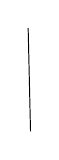
\begin{tikzpicture}[x=1cm,y=1cm]\draw[line width=.35pt] (0,0)--(.03,-1.31);\end{tikzpicture}}}
\uline{Corollary 2} Under the preceding conditions, we have

\[
\begin{array}{@{}l@{\qquad}l@{}}
(15) & {\color{red}\boxed{{\color{black}\displaystyle |\alpha_n u_1,\mathord{-}u_n)|\leq\frac1{n!}\lVert u_1\rVert\mathord{-}\,\mathord{-}\lVert u_n\rVert}}}
\end{array}
\]

(This also follows from the fact, already noted, that the coefficient $k_n$ of Chapter I, \S~1, N\textsuperscript{o} 2, proposition 1, is here equal to 1).

{\reversemarginpar\margin{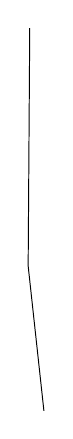
\begin{tikzpicture}[x=1cm,y=1cm]\draw[line width=.35pt] (0,0)--(-.02,-3.02)--(.18,-4.86);\end{tikzpicture}}}
\uline{Corollary 3} Let \deleted{$u\in L^1(E)$, where $E$ is a Hilbert space} \inserted{$u$ be a Fredholm operator on a} Hilbert space $E$. \deleted{Then,} If $u$ is a Fredholm operator, the same is true of $\overset{n}{\Lambda}u$, and we have

\[
\begin{array}{@{}l@{\qquad}l@{}}
(16) & \displaystyle \lVert\overset{n}{\Lambda}u\rVert_1=\alpha_n\deleted{\unsure{(\sqrt{u^*u})}}(|u|)\inserted{={\color{red}\underline{{\color{black}\alpha_n(\sqrt{\unsure{u^*u|u^*}})}}}}
\end{array}
\]

If $u$ is a Hilbert--Schmidt operator, the same is true of $\overset{n}{\Lambda}u$, and we have

\[
\begin{array}{@{}l@{\qquad}l@{}}
(\unsure{17|14}) & \displaystyle \lVert\overset{n}{\Lambda}u\rVert_2=\sqrt{\alpha_n(u^*u)}
\end{array}
\]

We have, if $u\in L^1(E)$, $\lVert\overset{n}{\Lambda}u\rVert_1=\operatorname{Tr}\deleted{\sqrt{\vphantom{(\overset{n}{\Lambda}u)^*}}}\bigl((\overset{n}{\Lambda}u)^*(\overset{n}{\Lambda}u)\bigr)^{1/2}$ (N\textsuperscript{o} 1, formula (22)), now, (proposition 1) we have $\deleted{\sqrt{\vphantom{(\overset{n}{\Lambda}u)^*}}}\bigl((\overset{n}{\Lambda}u)^*(\overset{n}{\Lambda}u)\bigr)^{1/2}=\overset{n}{\Lambda}\bigl((u^*u)^{1/2}\bigr)$, whence \deleted{(16) by virtue of (17)} \inserted{$\lVert\overset{n}{\Lambda}u\rVert_1=\operatorname{Tr}\overset{n}{\Lambda}((u^*u)^{1/2})=\alpha_n(\sqrt{u^*u})$} (by virtue of (14)).

\deleted{If $u\in L^2(E)$, \inserted{then} we still have, $(\overset{n}{\Lambda}u)^*(\overset{n}{\Lambda}u)=\overset{n}{\Lambda}(u^*u)$ \unsure{where we} \unsure{had} $u^*u\in L^1(E)$ \inserted{is a Fredholm operator} (whence $(\overset{n}{\Lambda}u)^*(\overset{n}{\Lambda}u)=\overset{n}{\Lambda}(u^*u)$ is $\in L^1(E)$, and $\overset{n}{\Lambda}u$ \unsure{consequently}}

If $u$ is a Hilbert--Schmidt operator, then $u^*u$ is a Fredholm operator (N\textsuperscript{o} 1, theorem~4), therefore $(\overset{n}{\Lambda}u)^*(\overset{n}{\Lambda}u)=\overset{n}{\Lambda}(u^*u)$ is a Fredholm operator, \deleted{and} therefore $\overset{n}{\Lambda}u$ is a Hilbert--Schmidt operator. We have (N\textsuperscript{o} 1, theorem~3, corollary 3)

\[
(\lVert\overset{n}{\Lambda}u\rVert_2)^2=\operatorname{Tr}(\overset{n}{\Lambda}u)^*(\overset{n}{\Lambda}u)=\alpha_n(u^*u)\qquad\text{(formula (14), whence (17))}
\]
{\reversemarginpar\margin{\unsure{79|75}}}
